\documentclass{article}
\usepackage[utf8]{inputenc}
\usepackage{amsmath}
\usepackage[colorlinks, linkcolor=blue, citecolor=blue, urlcolor=blue]{hyperref}
\usepackage[danish]{babel}
\usepackage{graphicx}

\title{Test dokument}
\author{Henrik}

\begin{document}
\maketitle

\tableofcontents

\section{Først overskrift}
\label{secFoersteOverskrift}
Dette er et lille test dokument, hvor der er henvisninger, overskrifter 
og lidt matematik.

\subsection{Underoverskrift}
\label{ssecUnderoverskrift}
Noget mere tekst efterfulgt af en formel.
\begin{align}
\label{eqnPythagoras}
a^2 + b^2 = c^2
\end{align}

\subsection{Endnu et afsnit}
I afsnit \ref{ssecUnderoverskrift} blev Pythagoras' læresætning 
\eqref{eqnPythagoras} præsenteret.

\section{Mere matematik}

\begin{align}
c
	& = \sqrt{a^2 + b^2}			\\
\frac{d}{dx} x^2
	& = 2x
\end{align}


\section{Nogle lister}

En punkt opstillet liste
\begin{itemize}
\item	bananer
\item	citroner
\item	æbler
\end{itemize}

En nummereret liste
\begin{enumerate}
\item	Cykle til bilka
\item	Handle ind
\item	Cykle hjem
\end{enumerate}

\section{Figurer}

Se på figur \ref{figTestFigure}.

\begin{figure}
\centering
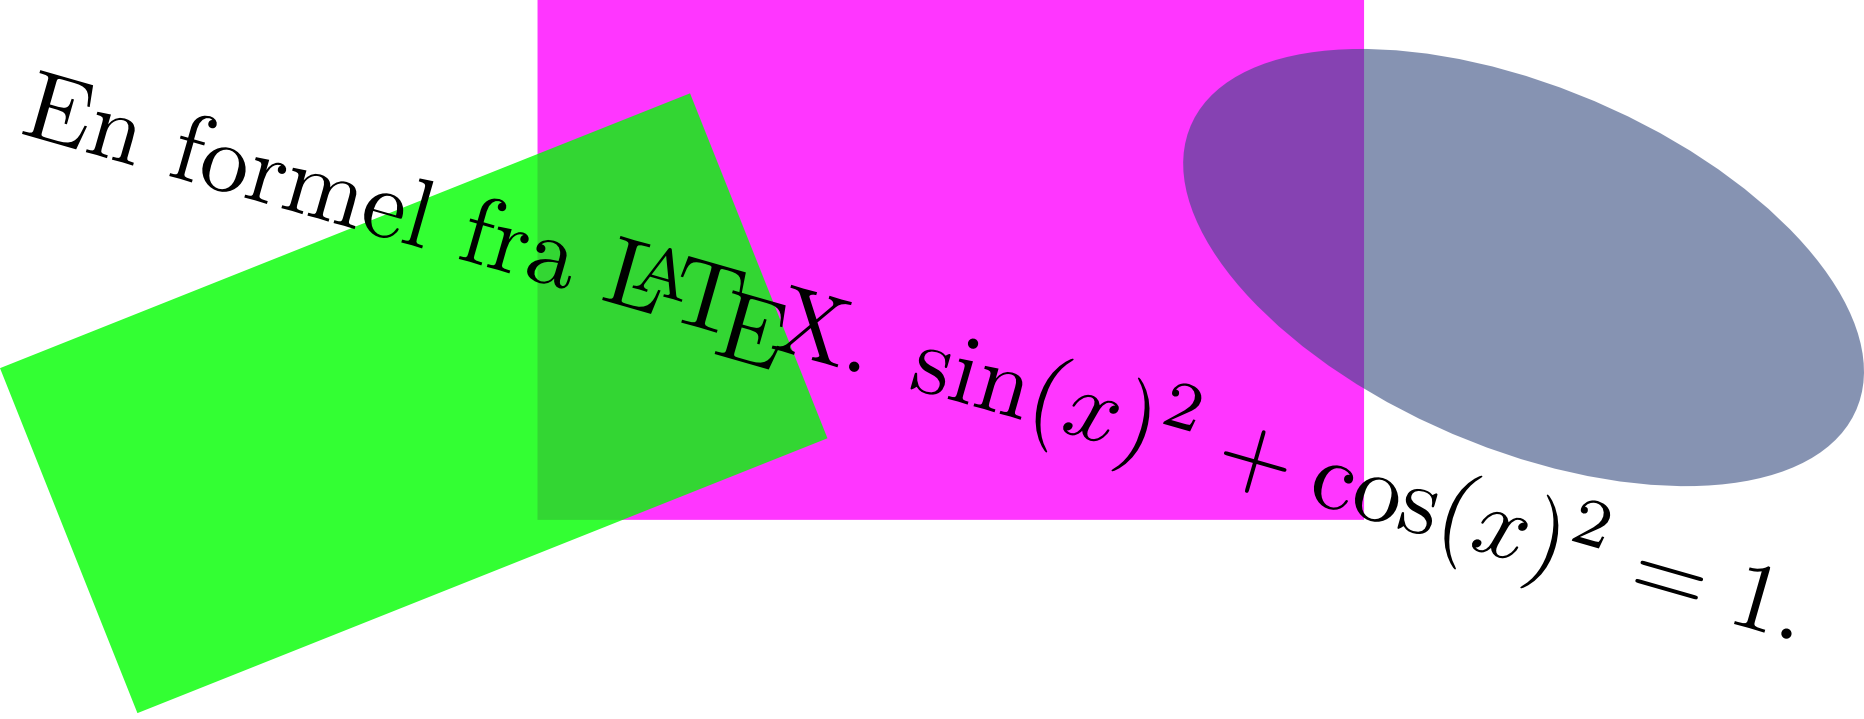
\includegraphics[width=6cm]{pic/figur.png}
\caption{Et png billede der er indsat.}
\label{figTestFigure}
\end{figure}

\end{document}